\documentclass[
12pt,
a4paper,
bibliography=totocnumbered, %Literaturverzereichnis als Eintrag ins Inhaltsverzeichnis
%twoside, %Zweiseitiger Druck
BCOR=1cm, %Platz zum Lochen
oneside, %Einseitiger Druck
]{scrartcl}

\usepackage{geometry}

\usepackage[default]{fontsetup}
%\usepackage[onehalfspacing]{setspace}

\usepackage[ngerman]{babel}
\usepackage[babel=true,german=quotes]{csquotes}

\usepackage{microtype}
\usepackage{mleftright}
%\newcommand{\Le}{\mleft}
%\newcommand{\Ri}{\mright}
\usepackage[no-script, no-scriptscript, no-inner, no-close]{innerscript}

% Mathepakete (unicode-math ersetzt amssymb, amsfonts etc.)
\usepackage{amsmath,amsthm}
\usepackage{mathtools}
\usepackage{fixdif,derivative}
\usepackage{physics2}
\usephysicsmodule{ab.legacy}

\usepackage{unicode-math}
\setmathfont{NewCMMath-Book}
\setmathfont{NewCMMath-Book}[range=cal, StylisticSet=1]
\setmathfont{NewCMMath-Book}[range=scr]

\usepackage{siunitx}
\sisetup{detect-weight=true, detect-family=true,locale=DE,range-phrase={\,bis\,},list-final-separator ={\,\linebreak[0] \text{und}\,},separate-uncertainty=true,per-mode = symbol-or-fraction}
%\SI[per-mode = fraction]{1}{\meter\per\second} erzwingt auch im Fließtext die Bruchdarstellung.
\DeclareSIUnit\curie{Ci}%Zusätzliche Einheit definieren

\usepackage{tabularx, booktabs, multirow}
\usepackage{array}
\usepackage{enumitem}
\usepackage{float}
\usepackage{graphicx}
\usepackage{xurl}

\usepackage[final]{pdfpages}
\usepackage{framed, color} %Framed: Paket, mittels dessen ein Rahmen um einen Bereich definiert werden kann. Color: Lässt Farbdarstellung in Schrift, Hintergrund etc. zu

\usepackage{scrlayer-scrpage} %Header für die KOMA-script-Klasse

%\usepackage[square,numbers]{natbib}
\usepackage{subfigure} %Mehrere Bilder in einer Figure-Umgebung

\usepackage[bookmarks,colorlinks=true]{hyperref}
\hypersetup{
	colorlinks,
	linktocpage,
	citecolor=black,
	filecolor=black,
	linkcolor=black,
	urlcolor=black,
	pdftitle=X,
	pdfauthor=JM-VS
}

\usepackage[backend=biber, style=chem-angew]{biblatex}
\addbibresource{lit.bib}

\numberwithin{equation}{section} % Die Nummerierung von Gleichungen bekommt die jeweilige Section-Nummer als Präfix

\setlength{\parindent}{0pt} %Einrücktiefe von neuen Absätzen
\setlength{\parskip}{6pt} %Abstand von Absätzen

\pagestyle{scrheadings}%Kopf und Fußzeilen
\ohead{\textbf{\GRUPPENNR\ - \VERSUCHSNR}} %Header oben links auf linker Seite (ungerade Seitenzahl) und oben rechts auf rechter Seite (gerade Seitenzahl), beinhaltet gruppennummer und Versuchskürzel. Im Fall eine einseitigen Dokuments: Header oben rechts
\ihead{\VerfasserEINS\;\&\;\VerfasserZWEI} %Header oben rechts auf linker Seite und oben links auf rechter Seite. Beinhaltet die Namen der Verfasser. Im Fall eine einseitigen Dokuments: Header oben links!
\ofoot{\thepage} %Footer unten links auf linker und unten rechts auf rechter Seite, enthält die jeweilige Seitenzahl. Im Fall eines einseitigen Elements: Footer unten rechts!
\cfoot{\empty} %Mittig unten im Footer soll nichts eingetragen werden
\ifoot{\empty} %Footer unten rechts auf linker und unten links auf rechter Seite. Hier ebenfalls leer.

\newcommand{\tz}{T_{\text{II}}}
\newcommand{\ts}{T_{\text{S}}}
\newcommand{\tgl}{T_{\text{gl}}}
\newcommand{\tgeg}{T_{\text{geg}}}
\newcommand{\omz}{\omega_{\text{II}}}
\newcommand{\omgl}{\omega_{\text{gl}}}
\newcommand{\omgeg}{\omega_{\text{geg}}}
\newcommand{\kB}{k_{\text{B}}}

% Hier können die individuellen Anpassungen vorgenommen werden, die sich auf das Titelblatt und die Kopfzeilen auswirken.

\newcommand{\VERSUCHSDATUM}{29.09.2025}
\newcommand{\PROTOKOLLDATUM}{\today}

\newcommand{\VerfasserEINS}{Julian Molt}
\newcommand{\MatNoEINS}{3803097}
\newcommand{\StudiengangEINS}{Physik}

\newcommand{\VerfasserZWEI}{Valentin Stopper}
\newcommand{\MatNoZWEI}{3774391}
\newcommand{\StudiengangZWEI}{Physik}

\newcommand{\BETREUER}{Julian Vollmer}
\newcommand{\GRUPPENNR}{A-016}

\newcommand{\VERSUCHSNR}{E24}
\newcommand{\VERSUCHSNAME}{Halbleiterdioden}

\newcommand{\lh}{\ell_{\mathrm{H}}}
\newcommand{\ls}{\ell_{\mathrm{S}}}


\begin{document}

\thispagestyle{empty}

\begin{titlepage}

	\begin{center}
		\Huge{\textbf{\VERSUCHSNR\ -- \VERSUCHSNAME}}\\
		\vspace{10mm}
		\Large{Protokoll zum Versuch des Physikalischen Praktikums I von \\ \textbf{\VerfasserEINS\;\& \VerfasserZWEI}}\\
		\vspace{10mm}
		\Large{Universität Stuttgart}\\
	\end{center}
	\vspace{1cm}
	\begin{center}
		\begin{tabular}{ll}
			\large{Verfasser:}		& \large{\VerfasserEINS\;(\StudiengangEINS),} \\
			& \large{\MatNoEINS} \\
			\vspace{0cm}\\
			& \large{\VerfasserZWEI\;(\StudiengangZWEI),} \\
			& \large{\MatNoZWEI} \\
			\vspace{0cm}\\
			\large{Gruppennummer:}	& \large{\GRUPPENNR} \\
			\vspace{0cm}\\
			\large{Versuchsdatum:}	& \large{\VERSUCHSDATUM} \\
			\vspace{0cm}\\
			\large{Betreuerin:}		& \large{\BETREUER}
		\end{tabular}
	\end{center}
	\vspace{15mm}

	\begin{center}
		Stuttgart, den \PROTOKOLLDATUM
	\end{center}

\end{titlepage}

\thispagestyle{empty}

\tableofcontents

\clearpage %Neue Seite, davor werden alle noch ausstehenden Grafiken/Tabellen platziert.

\renewcommand{\thepage}{\arabic{page}}
\setcounter{page}{1}


% Die erste eckige Klammer ist optional, die darin angegebene Bezeichnung steht im Inhaltsverzeichnis anstelle des hinteren (längeren) Namens.
\section[Versuchsziel]{Versuchsziel und Versuchsmethode}

In diesem Versuch werden Halbleiterdioden untersucht. Dazu werden die Kennlinien einer Silizium- und Germaniumdiode, einer Z-Diode und von zwei LEDs aufgezeichnet. Für die Z-Diode und die LEDs geschieht dies mithilfe eines Oszilloskops.

\section{Grundlagen}

Elektronen können in einem Atom diskrete Energieniveaus einnehmen. Nähern sich Atome einander an werden die Energieniveaus zu mehreren naheliegenden Energieniveaus aufgespalten. Innerhalb eines Einkristalls, mit vielen Wechselwirkenden Atomen, kommt es zu vielen Aufspaltungen, weshalb Naheliegende Energieniveaus zu Bändern zusammengefasst werden. Diese Bänder können von Elektronen besetzt werden, das höchste vollbesetzte Band heißt Valenzband. Das Band, welches energetisch über dem Valenzband liegt, heißt Leitungsband. Ein Kristall ist dann leitend, wenn er ein Teilweise besetztes Band hat, da die Elektronen nur dann ein höheres Energieniveau einnehmen können, um Energie zu übertragen. Als Bandlücke wird der Energiebereich zwischen Valenz- und Leitungsband bezeichnet. Die Energieniveaus innerhalb der Bandlücke können von Elektronen nicht eingenommen werden. Bei Isolatoren ist das Leitungsband unbesetzt und die Bandlücke groß, weshalb keine Elektronen ins Leitungsband kommen. Bei Halbleitern ist die Bandlücke kleiner, wodurch Elektronen unter geringer Energiezufuhr, wie bspw. Wärme oder Licht, ins Leitungsband gelangen können. Alternativ kann die Leitfähigkeit eines Halbleiters auch durch Dotierung verbessert werden. Bei der p-Dotierung werden in den Halbleiterkristall Atome niedriger Wertigkeit eingebracht, diese heißen Akzeptoren. Bei der n-Dotierung werden Atome höherer Wertigkeit eingebracht, sie heißen Donatoren. Dadurch entstehen freie Elektronen, bzw. Elektronenfehlstellen, die Strom leiten können.
Werden ein p- und ein n-Dotierter Halbleiter zusammengeführt, entsteht ein pn-Übergang. Im pn-Übergang bewegen sich Elektronen und Fehlstellen aufeinander zu und rekombinieren. Dadurch bleiben auf der p-dotierten Seite die negativ geladenen Atomrümpfe der Akzeptoren und auf der n-dotierten Seite die Positiv geladenen Rümpfe der Donatoren übrig. Beide werden nun nicht mehr ausgeglichen, weshalb sich ein elektrisches Feld von n- zu p-Seite bildet. Dieses stoppt weiteres Diffundieren der Elektronen und Fehlstellen, wodurch sich ein Gleichgewicht einstellt. Der mittlere Bereich des pn-Übergangs, in dem das Feld wirkt, heißt Raumladungszone.
Wird eine Spannung angelegt, mit negativem Pol an der n Seite und positivem an p , kann die Diffusion fortgesetzt werden, dann fließt Strom in Durchlassrichtung, unter ständiger Rekombination, bei der Energie frei wird. Werden die Pole am Halbleiter gewechselt sperrt die Diode und es fließt ausschließlich ein geringer Sperrstrom \(I_{\text{S}}\), welcher nicht durch Rekombination hervorgeht, sondern durch thermisch aktivierte Elektronen. Für  ideale pn-Übergänge von Dioden gilt die  Shockley'sche Beziehung
\begin{equation}
I=I_{\text{S}} \cdot \mleft[\exp\mleft( \frac{eU}{\kB T}\mright)-1 \mright]\,.
\end{equation}
Dabei steht \(e\) für die Elementarladung, \(\kB\) für die Boltzmankonstante, \(U\) für die Spannung und \(T\) für die Temperatur.
Bei einer sehr hohen Sperrspannung kann es zu einem hohen Sperrstrom, abweichend von der Shockleyschen Beziehung kommen. Der Hintergrund dafür ist einerseits der Zenereffekt, bei dem durch die Sperrspannung das Valenzband des P-dotierten Halbleiters und das Leitungsband des N-dotierten Halbleiters auf das selbe Energieniveau gehoben werden. Dadurch können Elektronen vom Valenz- direkt ins Leitungsband und ein Stromfluss wird möglich. Bei Zenerdioden, handelt es sich um stark dotierte Siliziumdioden, die sich genau diesen Effekt zu nutze machen.
Andererseits kann es zum Lawineneffekt kommen, bei dem freie, beschleunigte Elektronen andere Elektronen so schnell aus dem Gitter stoßen, dass keine Rekombination stattfinden kann. Diese stoßen wiederum gegen andere Elektronen, was einen schlagartigen Stromanstieg zu folge hat.
LEDs sind Dioden, bei denen Lichtquanten unter Rekombination entstehen.

Die elektrische Leitfähigkeit \(\sigma\) ist gegeben durch
\begin{equation}
	\sigma = \frac{1}{\rho}
\end{equation}
mit dem spezifischen Widerstand \(\rho\).
Der Widerstand \(R\) ist gegeben als
\begin{equation}
	R = \rho \cdot \frac{\ell}{A} \,,
\end{equation}
womit sich für die elektrische Leitfähigkeit
\begin{equation}\label{eq:Leitfähigkeit}
	\sigma = \frac{\ell}{RA}
\end{equation}
ergibt.
%\begin{figure}[H]
%	\centering{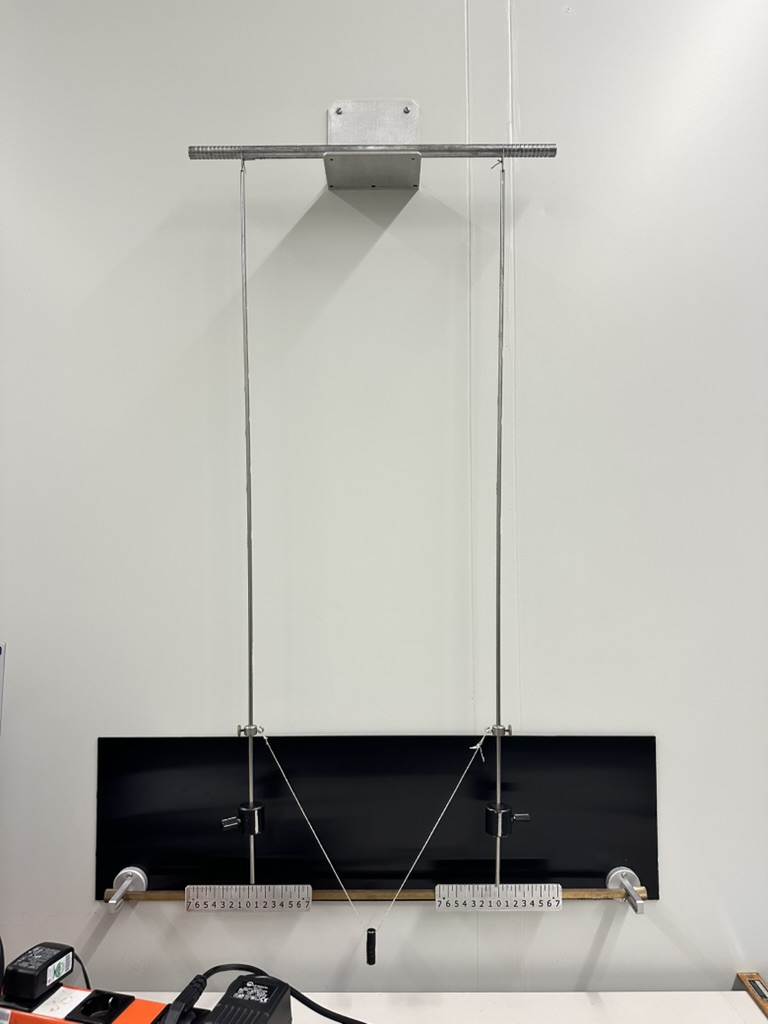
\includegraphics[width=0.4\textwidth]{Aufbau}}
%	\caption{Aufbau der Pendel, die hier bei \(\lh = \qty{70}{\centi\meter}\) gekoppelt sind.}
%	\label{fig:aufbau}
%\end{figure}

\section{Messwerte}

\begin{table}[H]
	\centering % damit die Tabelle trotzdem mittig steht
	\caption{Gemessene Spannung und Strom der Germanium-Diode.\label{tbl:GeDiode}}
	\begin{tabular}{ll}
		\toprule
		Spannung in \si{\milli\volt} & Strom in \si{\micro\ampere} \\
		\midrule
		\num{22,7}  & \num{0,06}  \\
		\num{100,2} & \num{11,9}  \\
		\num{152,0} & \num{55,5}  \\
		\num{199,3} & \num{182,3} \\
		\num{210,2} & \num{234,4} \\
		\num{220,2} & \num{292,3} \\
		\num{230,1} & \num{360}   \\
		\num{250,6} & \num{550}   \\
		\num{270,3} & \num{810}   \\
		\num{283,6} & \num{1050}  \\
		\num{320,3} & \num{1980}  \\
		\num{346,0} & \num{2990}  \\
		\num{366,0} & \num{4020}  \\
		\num{383,0} & \num{5020}  \\
		\num{397,0} & \num{5990}  \\
		\num{410,0} & \num{6990}  \\
		\num{422,0} & \num{8000}  \\
		\bottomrule
	\end{tabular}
\end{table}

\begin{table}[H]
	\centering % damit die Tabelle trotzdem mittig steht
	\caption{Gemessene Spannung und Strom der Silizium-Diode.\label{tbl:SiDiode}}
	\begin{tabular}{ll}
		\toprule
		Spannung in \si{\milli\volt} & Strom in \si{\micro\ampere} \\
		\midrule
		\num{99,4}  & \num{0,2} \\
		\num{155,2}  & \num{0,2} \\
		\num{208,2}  & \num{0,1} \\
		\num{304,6}  & \num{1}  \\
		\num{400}  & \num{11,8}  \\
		\num{452}  & \num{47,3}  \\
		\num{500}  & \num{149,3} \\
		\num{520}  & \num{238,9} \\
		\num{539}  & \num{355} \\
		\num{580}  & \num{820} \\
		\num{598}  & \num{1220} \\
		\num{623}  & \num{2020} \\
		\num{641}  & \num{2970} \\
		\num{655}  & \num{3980} \\
		\num{666}  & \num{5050} \\
		\num{674}  & \num{6020} \\
		\num{681}  & \num{7020} \\
		\num{687}  & \num{8010} \\
		\bottomrule
	\end{tabular}
\end{table}

\begin{table}[H]
	\centering % damit die Tabelle trotzdem mittig steht
	\caption{Gemessene Spannung und Strom der Silizium-Diode.\label{tbl:TempSi}}
	\begin{tabular}{lrr}
		\toprule
		Temperatur & Spannung in \si{\milli\volt} & Strom in \si{\micro\volt} \\
		\midrule
		\enquote{kalt} & \num{517} & \num{199,6} \\
		\enquote{warm} & \num{510} & \num{204,6}\\
		\bottomrule
	\end{tabular}
\end{table}

\begin{table}[H]
	\centering % damit die Tabelle trotzdem mittig steht
	\caption{Gemessene Spannung und Strom der Silizium-Diode.\label{tbl:TempGe}}
	\begin{tabular}{lrr}
		\toprule
		Temperatur & Spannung in \si{\milli\volt} & Strom in \si{\micro\volt} \\
		\midrule
		\enquote{kalt} & \num{201,9} & \num{200,4} \\
		\enquote{warm} & \num{191,5} & \num{207,4} \\
		\bottomrule
	\end{tabular}
\end{table}

\begin{table}[H]
	\centering % damit die Tabelle trotzdem mittig steht
	\caption{Gemessene Spannung und Strom der Silizium-Diode.\label{tbl:SiSperr}}
	\begin{tabular}{ll}
		\toprule
		Spannung in \si{\milli\volt} & Strom in \si{\micro\volt} \\
		\midrule
		\num{0,517} & \num{0,2} \\
		\num{1,061} & \num{0,3} \\
		\num{2,032} & \num{0,4} \\
		\num{3,220} & \num{0,5} \\
		\num{4,060} & \num{0,6} \\
		\num{5,120} & \num{0,7} \\
		\num{6,070} & \num{0,8} \\
		\num{7,060} & \num{0,9} \\
		\num{7,770} & \num{1,0} \\
		\bottomrule
	\end{tabular}
\end{table}

\begin{table}[H]
	\centering % damit die Tabelle trotzdem mittig steht
	\caption{Gemessene Spannung und Strom der Germanium-Diode.\label{tbl:GeSperr}}
	\begin{tabular}{ll}
		\toprule
		Spannung in \si{\milli\volt} & Strom in \si{\micro\volt} \\
		\midrule
		\num{0,518} & \num{0,7} \\
		\num{1,014} & \num{0,8} \\
		\num{1,527} & \num{0,9} \\
		\num{2,996} & \num{1,1} \\
		\num{4,050} & \num{1,2} \\
		\num{5,200} & \num{1,4} \\
		\num{6,000} & \num{1,5} \\
		\num{6,810} & \num{1,6} \\
		\num{7,510} & \num{1,7} \\
		\num{7,770} & \num{1,0} \\
		\bottomrule
	\end{tabular}
\end{table}

\section{Auswertung}

Die Leitfähigkeit der kalten Diode beträgt nach \autoref{eq:Leitfähigkeit}
\begin{equation}
	\sigma_{\text{k}} = \frac{\ell}{R_{\text{k}}A}
\end{equation}
und für die Warme
\begin{equation}
	\sigma_{\text{w}} = \frac{\ell}{R_{\text{w}}A} \,.
\end{equation}

Somit ist die prozentuale Änderung der Leitfähigkeit \(\Delta \sigma\) für die Silizium-Diode
\begin{align*}
	\Delta \sigma &= \frac{\sigma_{\text{w}}}{\sigma_{\text{k}}} -1 = \frac{\frac{\ell}{R_{\text{w}}A}}{\frac{\ell}{R_{\text{k}}A}} -1 = \frac{R_{\text{k}}}{R_{\text{w}}} -1 = \frac{\frac{U_{\text{k}}}{I_\text{k}}}{\frac{U_{\text{w}}}{I_{\text{w}}}} -1\\
	&= \frac{\frac{\qty{517e-3}{\volt}}{\qty{199,6e-6}{\ampere}}}{\frac{\qty{510e-3}{\volt}}{\qty{204,6e-6}{\ampere}}} -1 = \frac{\qty{2492,67}{\ohm}}{\qty{2590,18}{\ohm}} -1\\
	&= \qty{-4}{\percent} \,.
\end{align*}
Für die Germanium-Diode ergibt sich eine Änderung von \qty{-8}{\percent}.

Bei Messung der der Sperrkennlinien der beiden Dioden wird muss auch der Fehlerstrom \(I_{\text{err}}\) einberechnet werden. Vorher war dieser zu vernachlässigen, da der Innenwiderstand des Voltmeters sehr hoch ist, der der Diode in Durchlassrichtung aber sehr klein. In Sperrrichtung ist der Widerstand der Diode groß, was bedeutet, dass sich der Strom mehr auf die Diode und das Spannungsmessgerät aufteilt. Er berechnet sich folgendermaßen:
\begin{equation*}
	I_{\text{err}} = \frac{U}{R_{\text{Messgerät}}}
\end{equation*}
Hierbei wird angenommen, dass der Widerstand des Amperemeters vernachlässigbar klein ist und somit die Spannung, die vom Voltmeter angezeigt wird, die ist, die über die Diode abfällt.

Der Fehlerstrom muss vom gemessenen Strom des Amperemeters abgezogen werden.
\begin{figure}[H]
	\centering{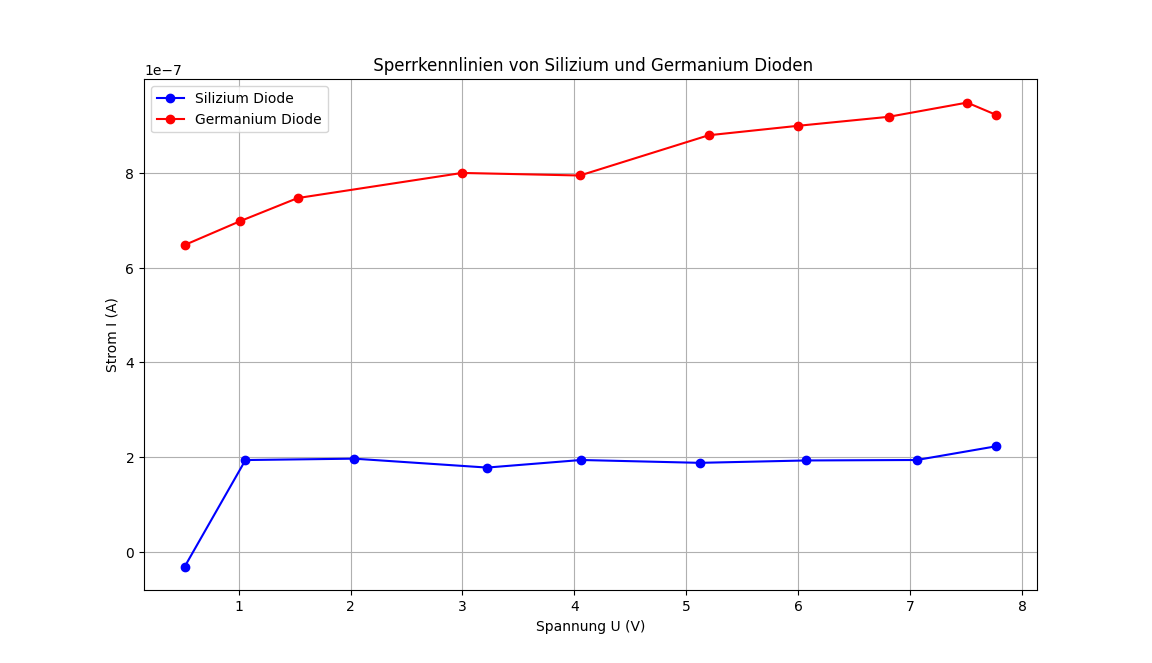
\includegraphics[width=0.9\textwidth]{SperrstromSiGe.png}}
	\caption{Sperrkennlinien der Si- und Ge-Dioden.}
	\label{fig:Sperrkennlinien}
\end{figure}

Die Kennlinie der Z-Diode wird mit einem Oszilloskop gemessen und kann in einem linearen Diagramm dargestellt werden.
\begin{figure}[H]
	\centering{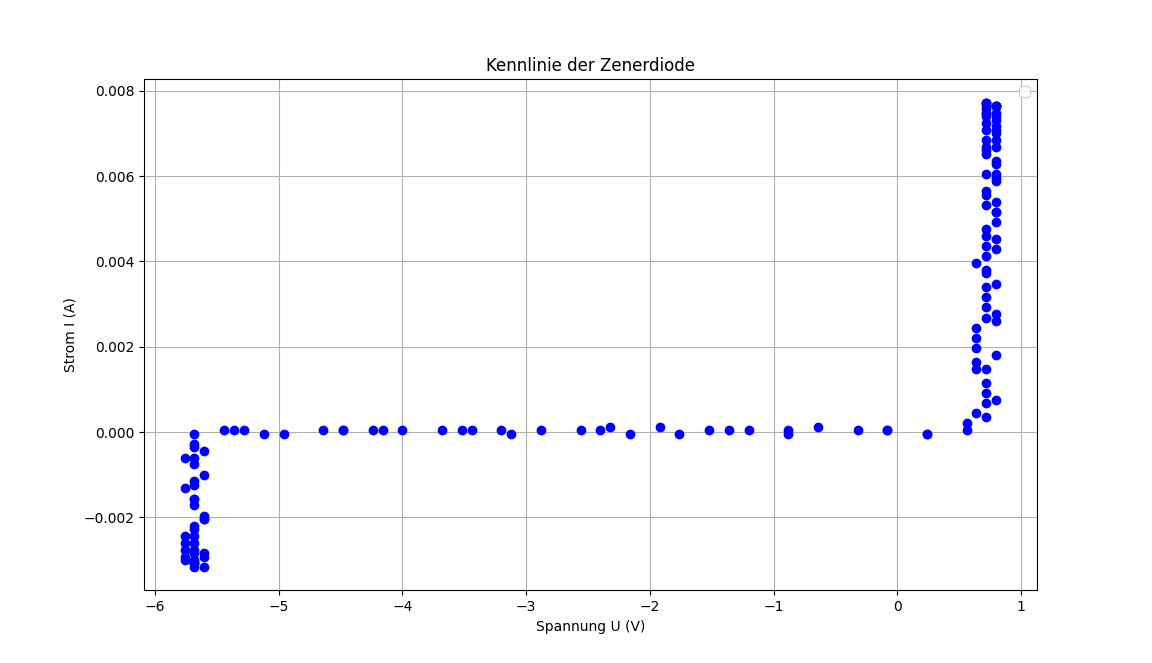
\includegraphics[width=0.9\textwidth]{KennlinieZ.png}}
	\caption{Kennlinie der Z-Diode.}
	\label{fig:KennlinieZ}
\end{figure}

ZENEREFFEKT ERKLÄREN

Die Kennlinien einer roten und blauen LED werden ebenfalls mit einem Oszilloskop aufgenommen führen auf die folgenden Kennlinien.
\begin{figure}[H]
	\centering{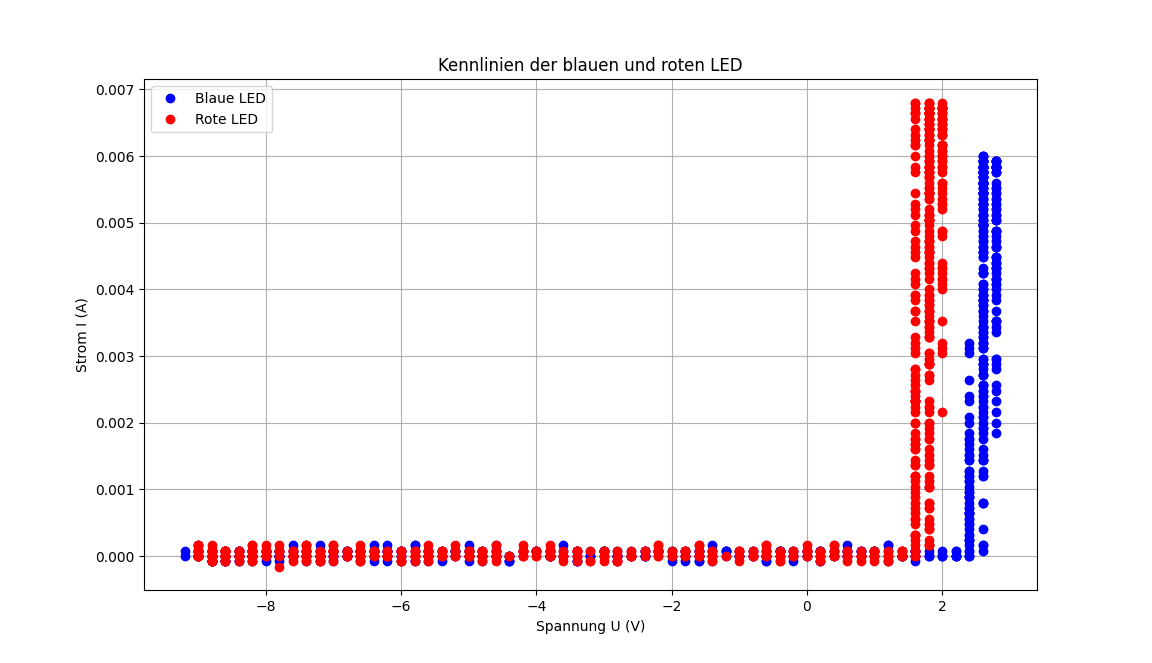
\includegraphics[width=0.9\textwidth]{KennlinieLED.png}}
	\caption{Kennlinie einer roten und einer blauen LED.}
	\label{fig:KennlinieLED}
\end{figure}

Es ist deutlich zu erkennen, dass die rote LED eine niedrigere Schwellenspannung besitz, als die Blaue. Das liegt am unterschiedlichen Aufbaue beider Dioden. Bei beiden Dioden wird die Lichtemission dadurch ausgelöst, dass, sobald die LED in Durchlassrichtung geschaltet ist, Elektronen im Leiterband von der n-dotierten Seite auf die p-dotierte Seite gelangen und dort unter Emission von Photonen mit den Deffektelektronen rekombinieren.

Ein Elektron hat die Energie
\begin{equation*}
	E = e \cdot U \,.
\end{equation*}
Als Näherung kann man annehmen dass diese Energie vollständig als Licht emittiert wird. Die Energie von Licht mit der Wellenlänge \(\lambda\) ist
\begin{equation*}
	E_{\L} = \frac{hc}{\lambda}
\end{equation*}
mit dem Planck'schen Wirkungsquantum \(h\) und der Lichtgeschwindigkeit \(c\).
Dann lautet die Relation zwischen angelegter Spannung und Wellenlänge
\begin{equation*}
	U = \frac{hc}{e\lambda}
\end{equation*}
%\section{Fehlerrechnung}
Für eine rote Diode mit einer Schwellspannung von ca. \qty{1,7}{\volt} ergibt sich somit eine Wellenlänge von
\begin{equation*}
	\lambda = \frac{hc}{eU} = \frac{bumms einsetzen}{\cdot \qty{1,7}{\volt}}
\end{equation*}

\section{Zusammenfassung}

\begin{thebibliography}{999}
	\bibitem{Quelle} Versuchsanleitung zu \emph{E24 -- Halbleiterdioden} (Abgerufen am 29.09.2025).
	Online verfügbar unter: \url{https://www3.physik.uni-stuttgart.de/studium/praktika/ap/pdf_dateien/E24.pdf}
\end{thebibliography}

%\printbibliography
\section{Anhang}

%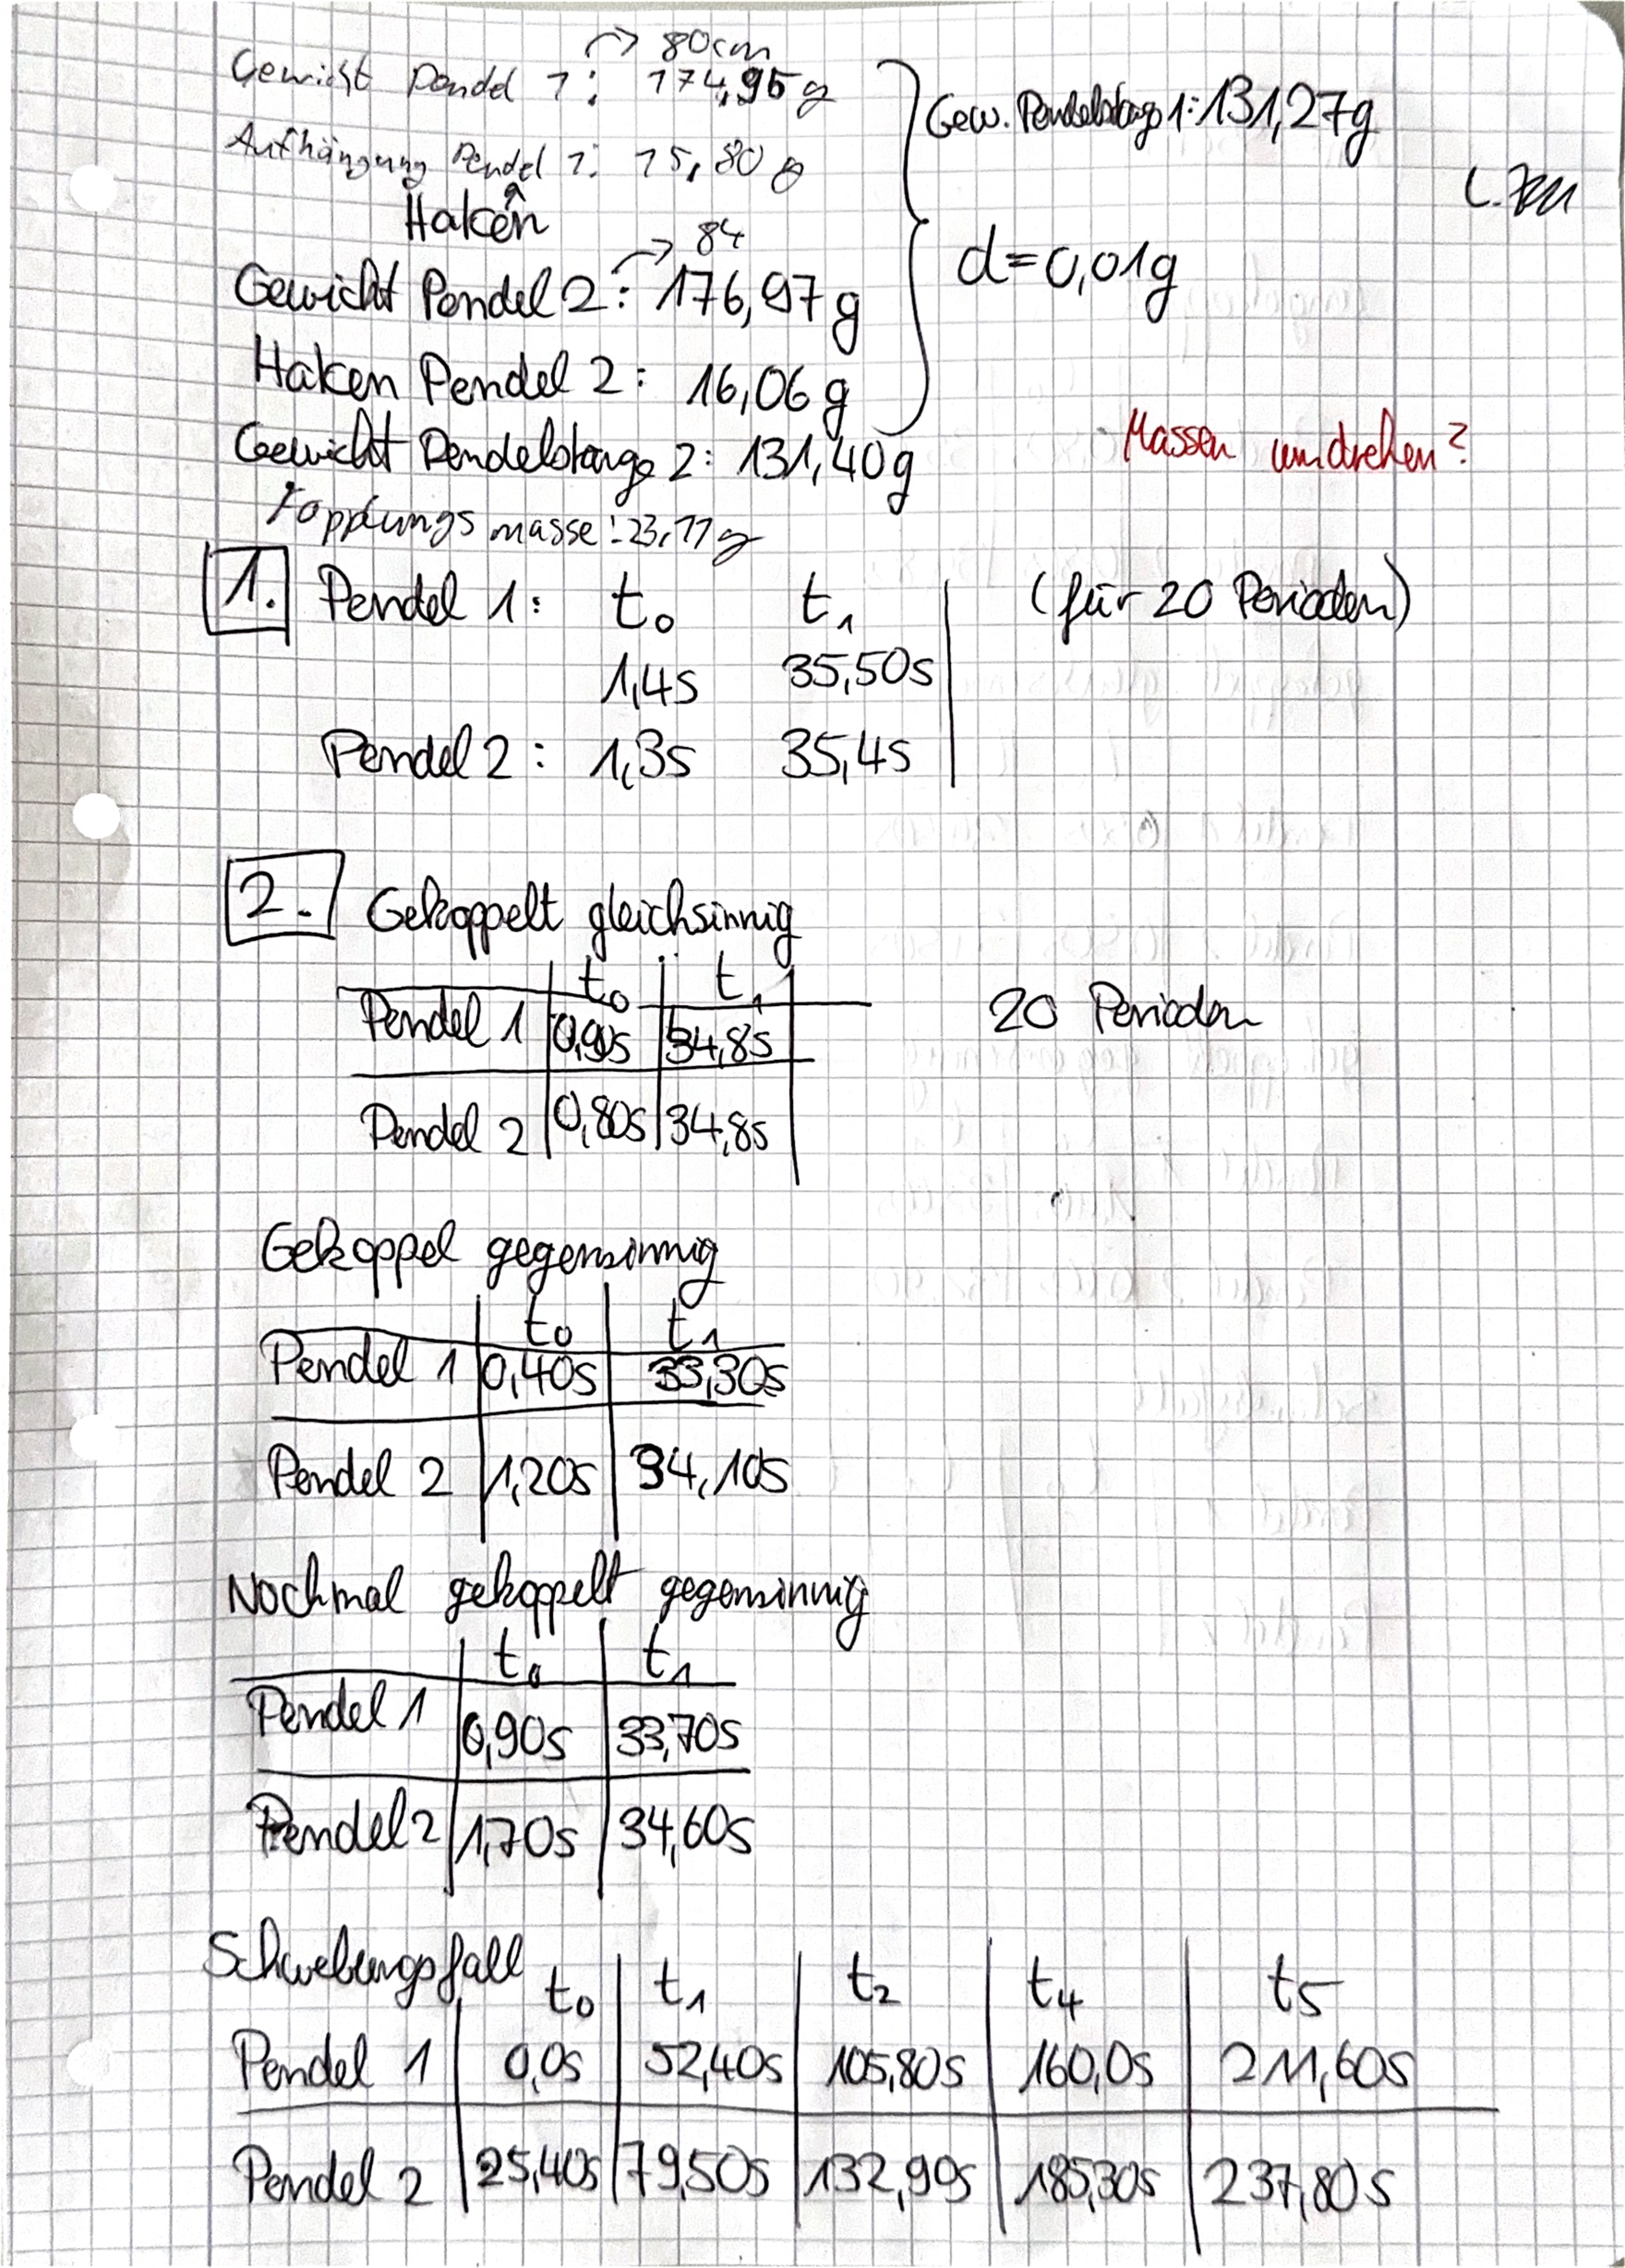
\includepdf[pages=-]{Messprotokoll.pdf}

\end{document}